\documentclass[final]{beamer}
\usepackage[orientation=landscape,size=custom,width=121.92,height=91.44,scale=1.15]{beamerposter}
\usepackage{mf_poster_style}

\graphicspath{{./}}

\renewcommand{\bodyfont}{\fontsize{33}{39.8}\selectfont}
\renewcommand{\capfont}{\fontsize{27.5}{33.1}\selectfont}

\renewcommand{\contentstart}{9.67cm}
\setlength{\colheight}{68.45cm}

\hyphenpenalty=10000
\exhyphenpenalty=10000
\tolerance=9999
\emergencystretch=3em

\newcommand{\figcaptionc}[1]{%
  \par\vspace{0.20cm}
  {\centering\capfont\color{DarkGrey} #1\par}%
}

% References + Acknowledgements + two QR panels (code, checkpoints).
\newcommand{\gatefooter}[2]{%
\begin{tikzpicture}[remember picture,overlay]
  \node[anchor=north west,inner sep=0pt] at
    ([xshift=\sidemargin,yshift=-83.9cm]current page.north west) {%
    \begin{minipage}[t]{\textwidth}
    \begin{columns}[T,totalwidth=\textwidth]
      \begin{column}{0.44\textwidth}
        {\headfont\bfseries\Large\color{AggieMaroon} References}\\[0.25cm]
        {\small\raggedright\color{DarkGrey} #1\par}
      \end{column}
      \begin{column}{0.33\textwidth}
        {\headfont\bfseries\Large\color{AggieMaroon} Acknowledgements}\\[0.25cm]
        {\small\raggedright\color{DarkGrey} #2\par}
      \end{column}
      \begin{column}{0.19\textwidth}
        \setqrboxw\vspace*{0.56cm}\par
        \hfill
        \begin{minipage}[t]{\qrboxw}\qrpanel{https://github.com/sheikhahnaf/matgen-BO}{Code}\end{minipage}%
        \hspace{0.9cm}%
        \begin{minipage}[t]{\qrboxw}\qrpanel{https://huggingface.co/SheikhAhnaf/apu-synthesizability-checkpoints}{Checkpoints}\end{minipage}%
        \hspace*{0.4cm}
      \end{column}
    \end{columns}
    \end{minipage}};
\end{tikzpicture}%
}

\begin{document}
\begin{frame}[t]

\posterchrome{}{0cm}{0cm}{10}

\posterheader
  {Surrogate-Gated Diffusion and Foundation-Model Embeddings for Bayesian Materials Design}
  {\textbf{Sk Md Ahnaf Akif Alvi}$^{1,2}$, Jan Janssen$^{3}$, Danny Perez$^{4}$,
   Douglas Allaire$^{5}$, Raymundo Arr\'{o}yave$^{1,5,6}$}
  {$^{1}$Materials Science and Engineering, $^{5}$Mechanical Engineering, $^{6}$Industrial and Systems Engineering, Texas A\&M University \quad
   $^{2}$Theoretical Division and $^{4}$X Computational Physics Division, Los Alamos National Laboratory \quad
   $^{3}$Max Planck Institute for Sustainable Materials}

\vspace*{\contentstart}

\begin{columns}[T,totalwidth=\textwidth]

%======================= COLUMN 1 (left) =======================
\begin{postercol}{\colw\textwidth}

\begin{posterbox}{Motivation}
\justifying
Diffusion priors fine-tuned by reinforcement learning propose crystals
faster than an oracle can score them. A surrogate placed before the
oracle only needs to rank candidates to decide which few deserve an
evaluation.

\vspace{0.45cm}
\begin{center}
\impactnumber[64]{3}{diffusion priors}
\impactnumber[64]{4}{oracle calls per cycle}
\impactnumber[64]{8{,}640}{benchmark fits}
\end{center}
\end{posterbox}

\vfill

\begin{posterbox}{The Gated Loop}
\centering
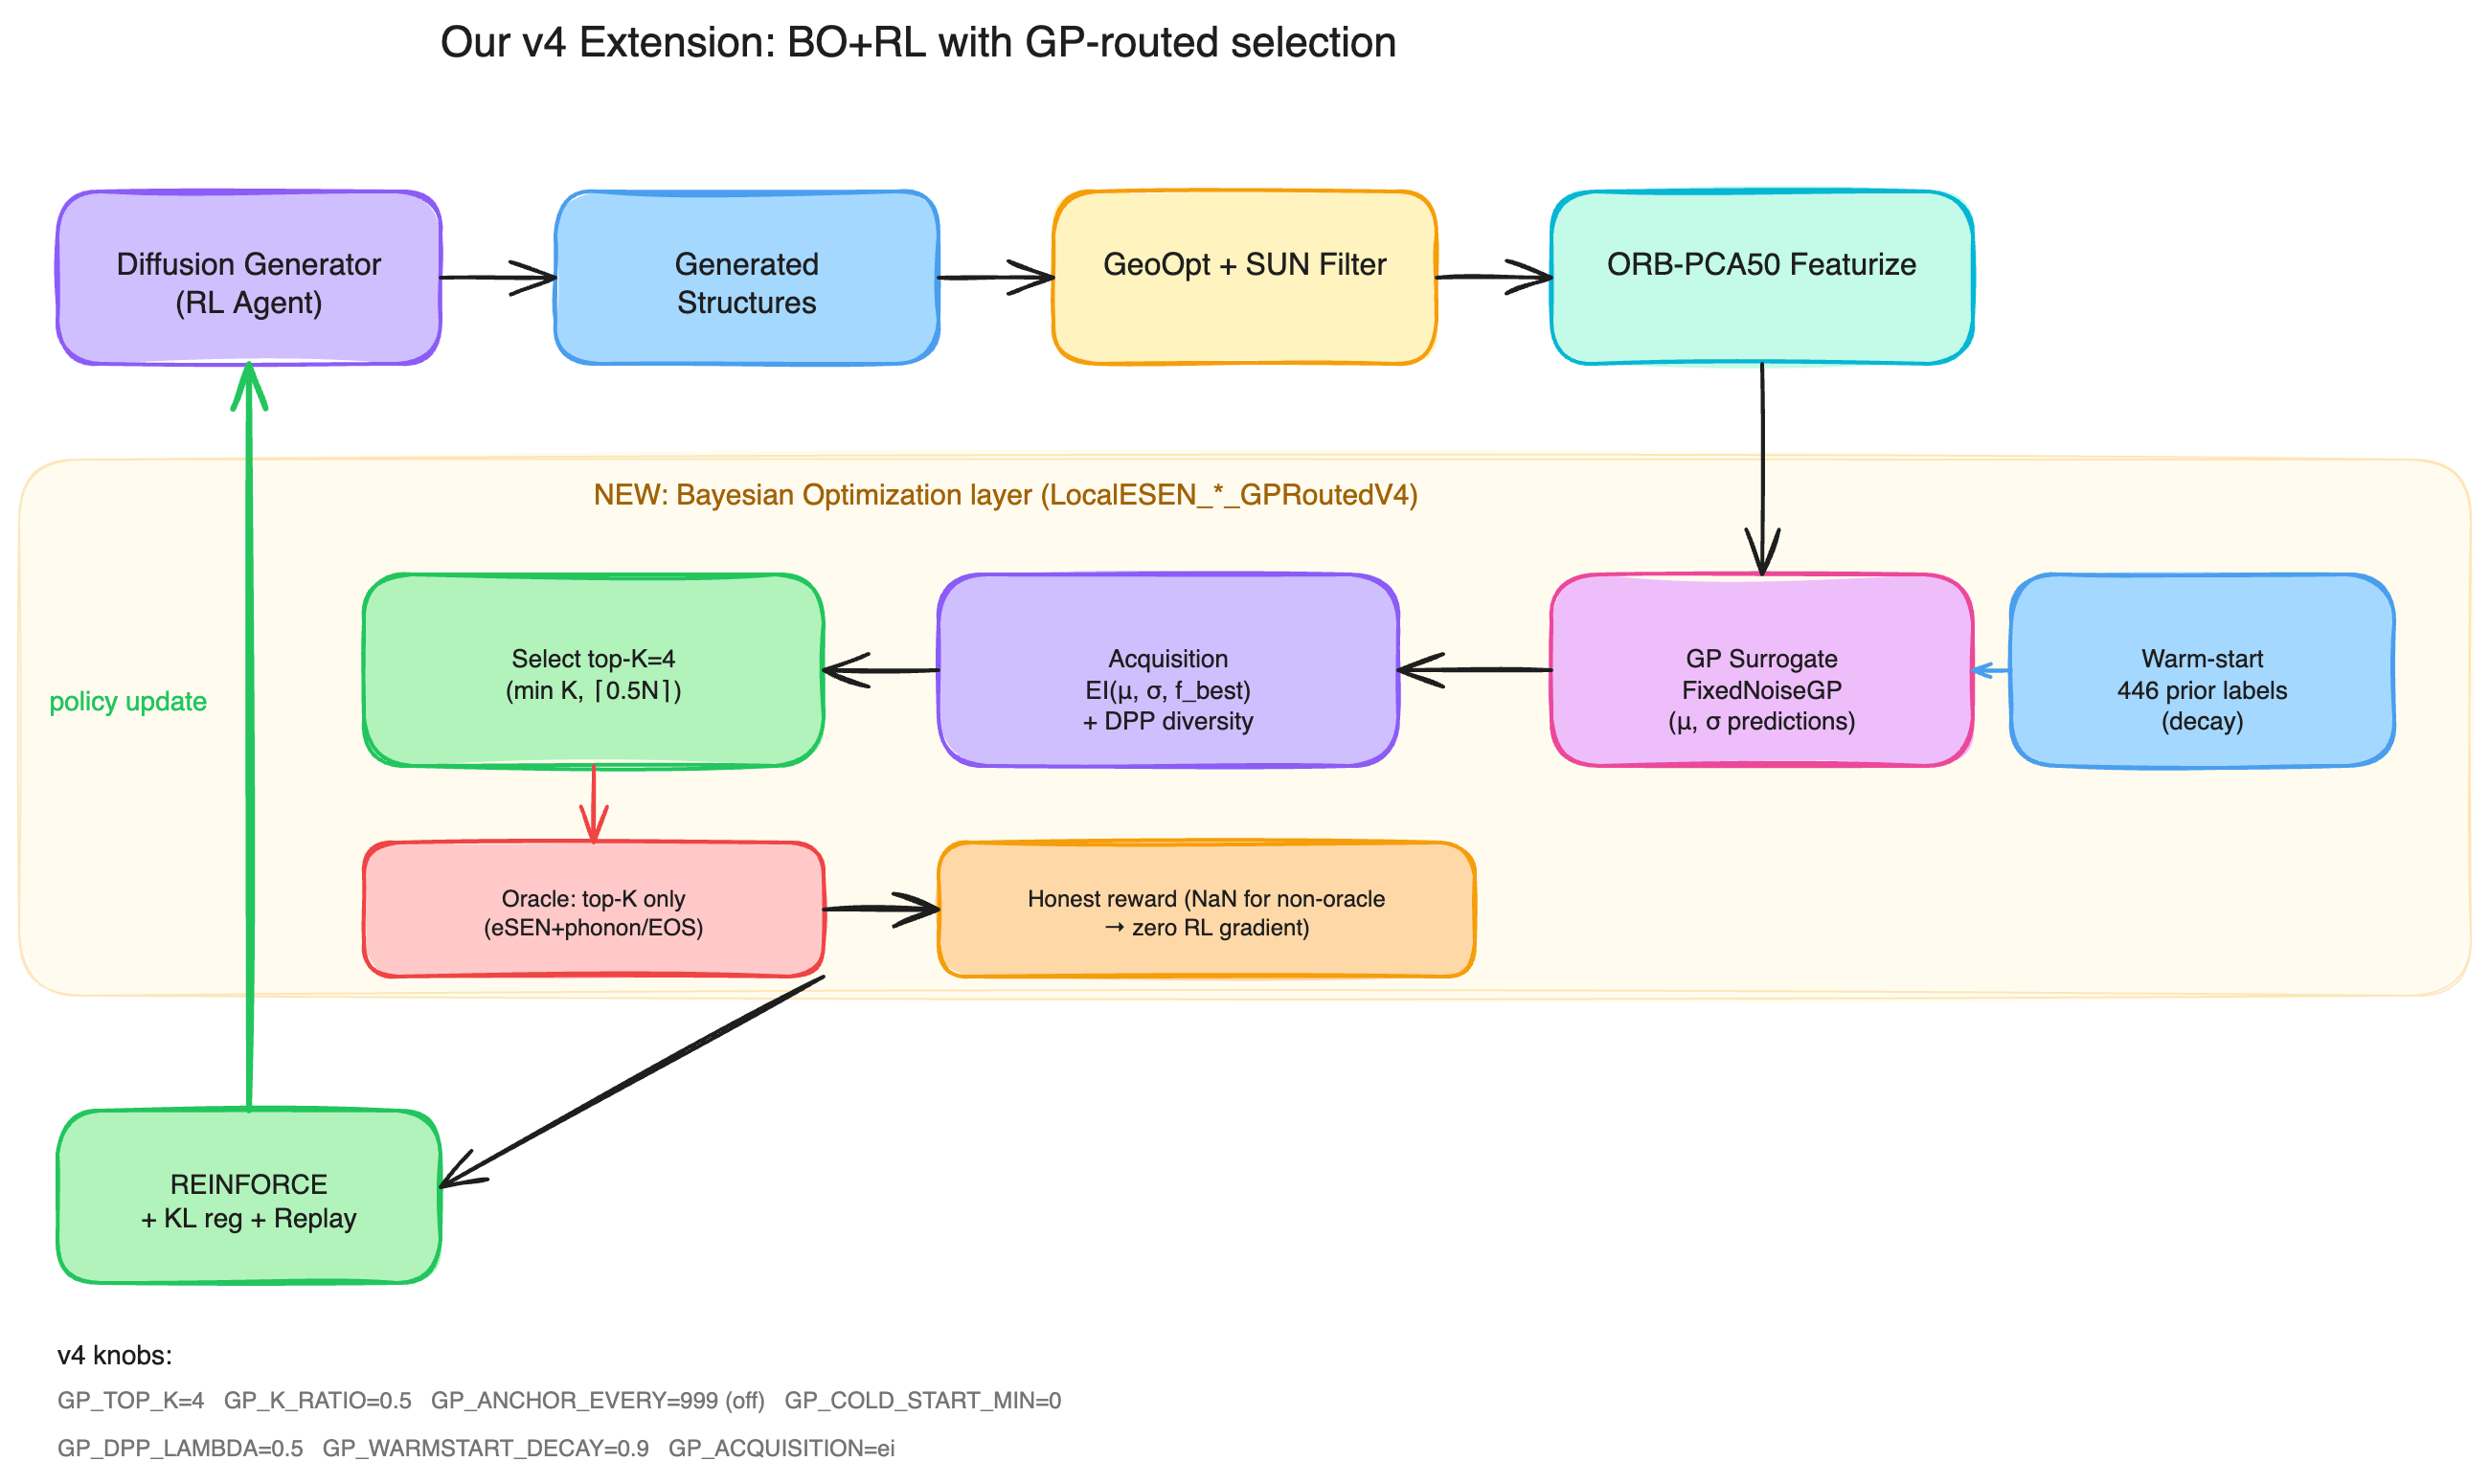
\includegraphics[width=\linewidth]{figs/fig_closed_loop_pipeline.png}

\vspace{0.35cm}
\justifying
Stable, unique and novel survivors are featurized with ORB and scored by
a Gaussian process; Expected Improvement with a diversity term sends the
top four to the oracle. The rest carry no reward, so the surrogate's
choice is the only training signal.
\end{posterbox}


\vfill

\begin{posterbox}{Choosing the Surrogate}
\centering
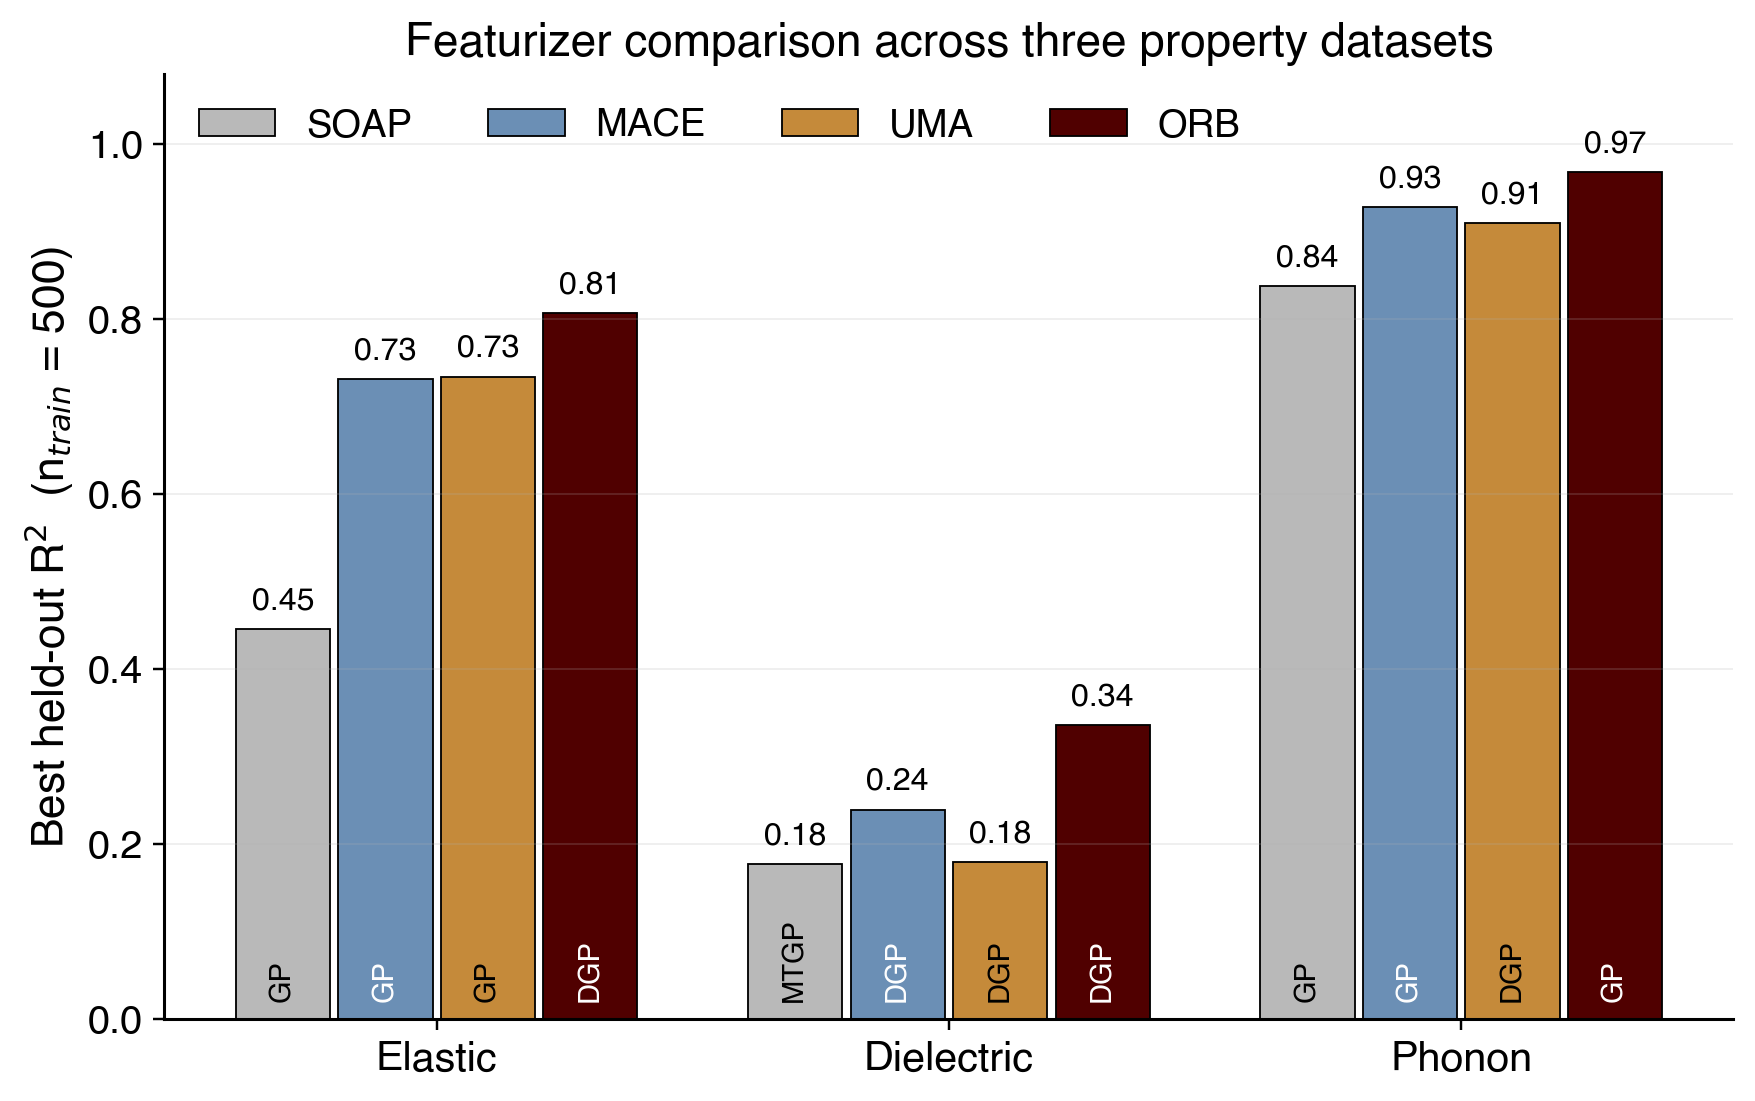
\includegraphics[width=0.76\linewidth]{figs/fig_benchmark_poster.png}

\vspace{0.35cm}
\justifying
Across mechanical, electronic and vibrational datasets, pretrained ORB
embeddings give the highest held-out accuracy; with a Gaussian process
on 50 principal components they define the gate.
\end{posterbox}

\end{postercol}

%======================= COLUMN 2 (center) =======================
\begin{postercol}{\midcolw\textwidth}

\begin{posterbox}[left=0.9cm,right=0.9cm]{Discovery Against Oracle Cost}
\centering
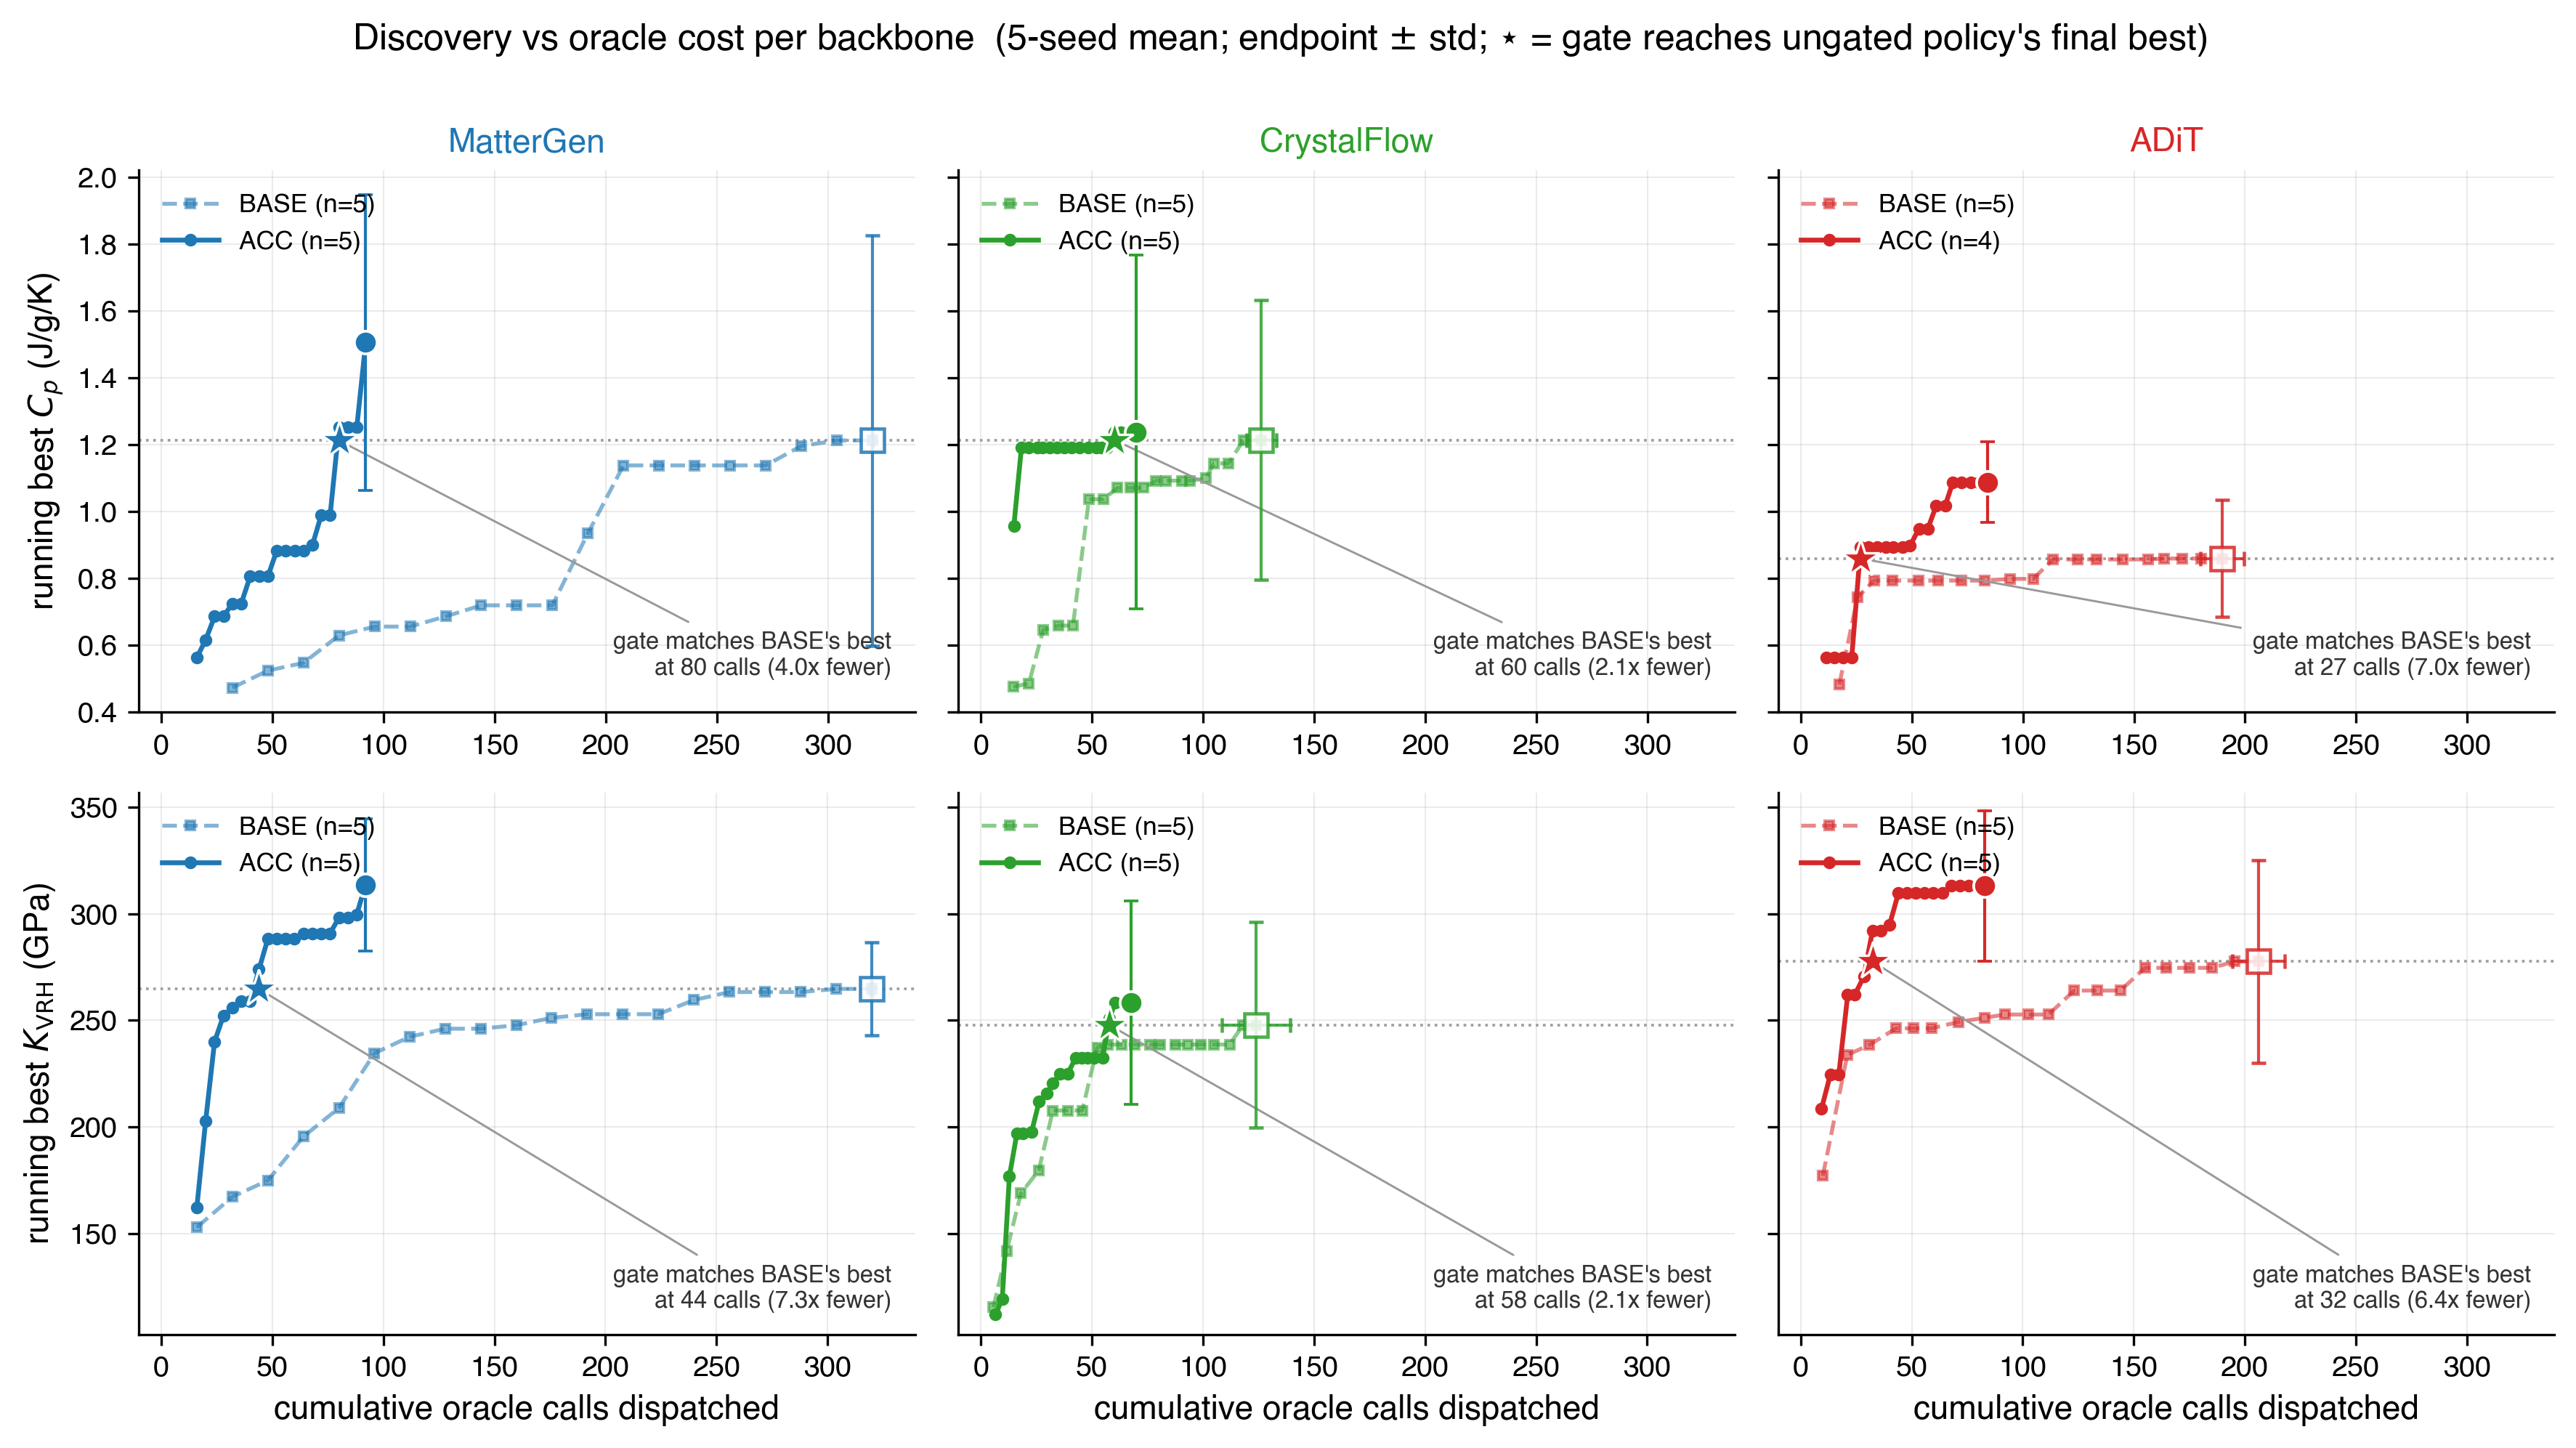
\includegraphics[width=0.90\linewidth]{figs/fig_value_cost_backbones_dispatched.png}

\vspace{0.35cm}
\justifying
Running best property against cumulative oracle calls for MatterGen,
CrystalFlow and ADiT, heat capacity (top) and bulk modulus (bottom),
five seeds per cell. The gated policy (solid) reaches the ungated
end-of-run best (star) with 2.1--7.3 times fewer oracle calls in all six
cells, and caps the budget at 92 calls per 20-cycle run.
\end{posterbox}

\vfill

\begin{posterbox}[left=0.9cm,right=0.9cm]{Selection, Not Budget, Drives Discovery}
\centering
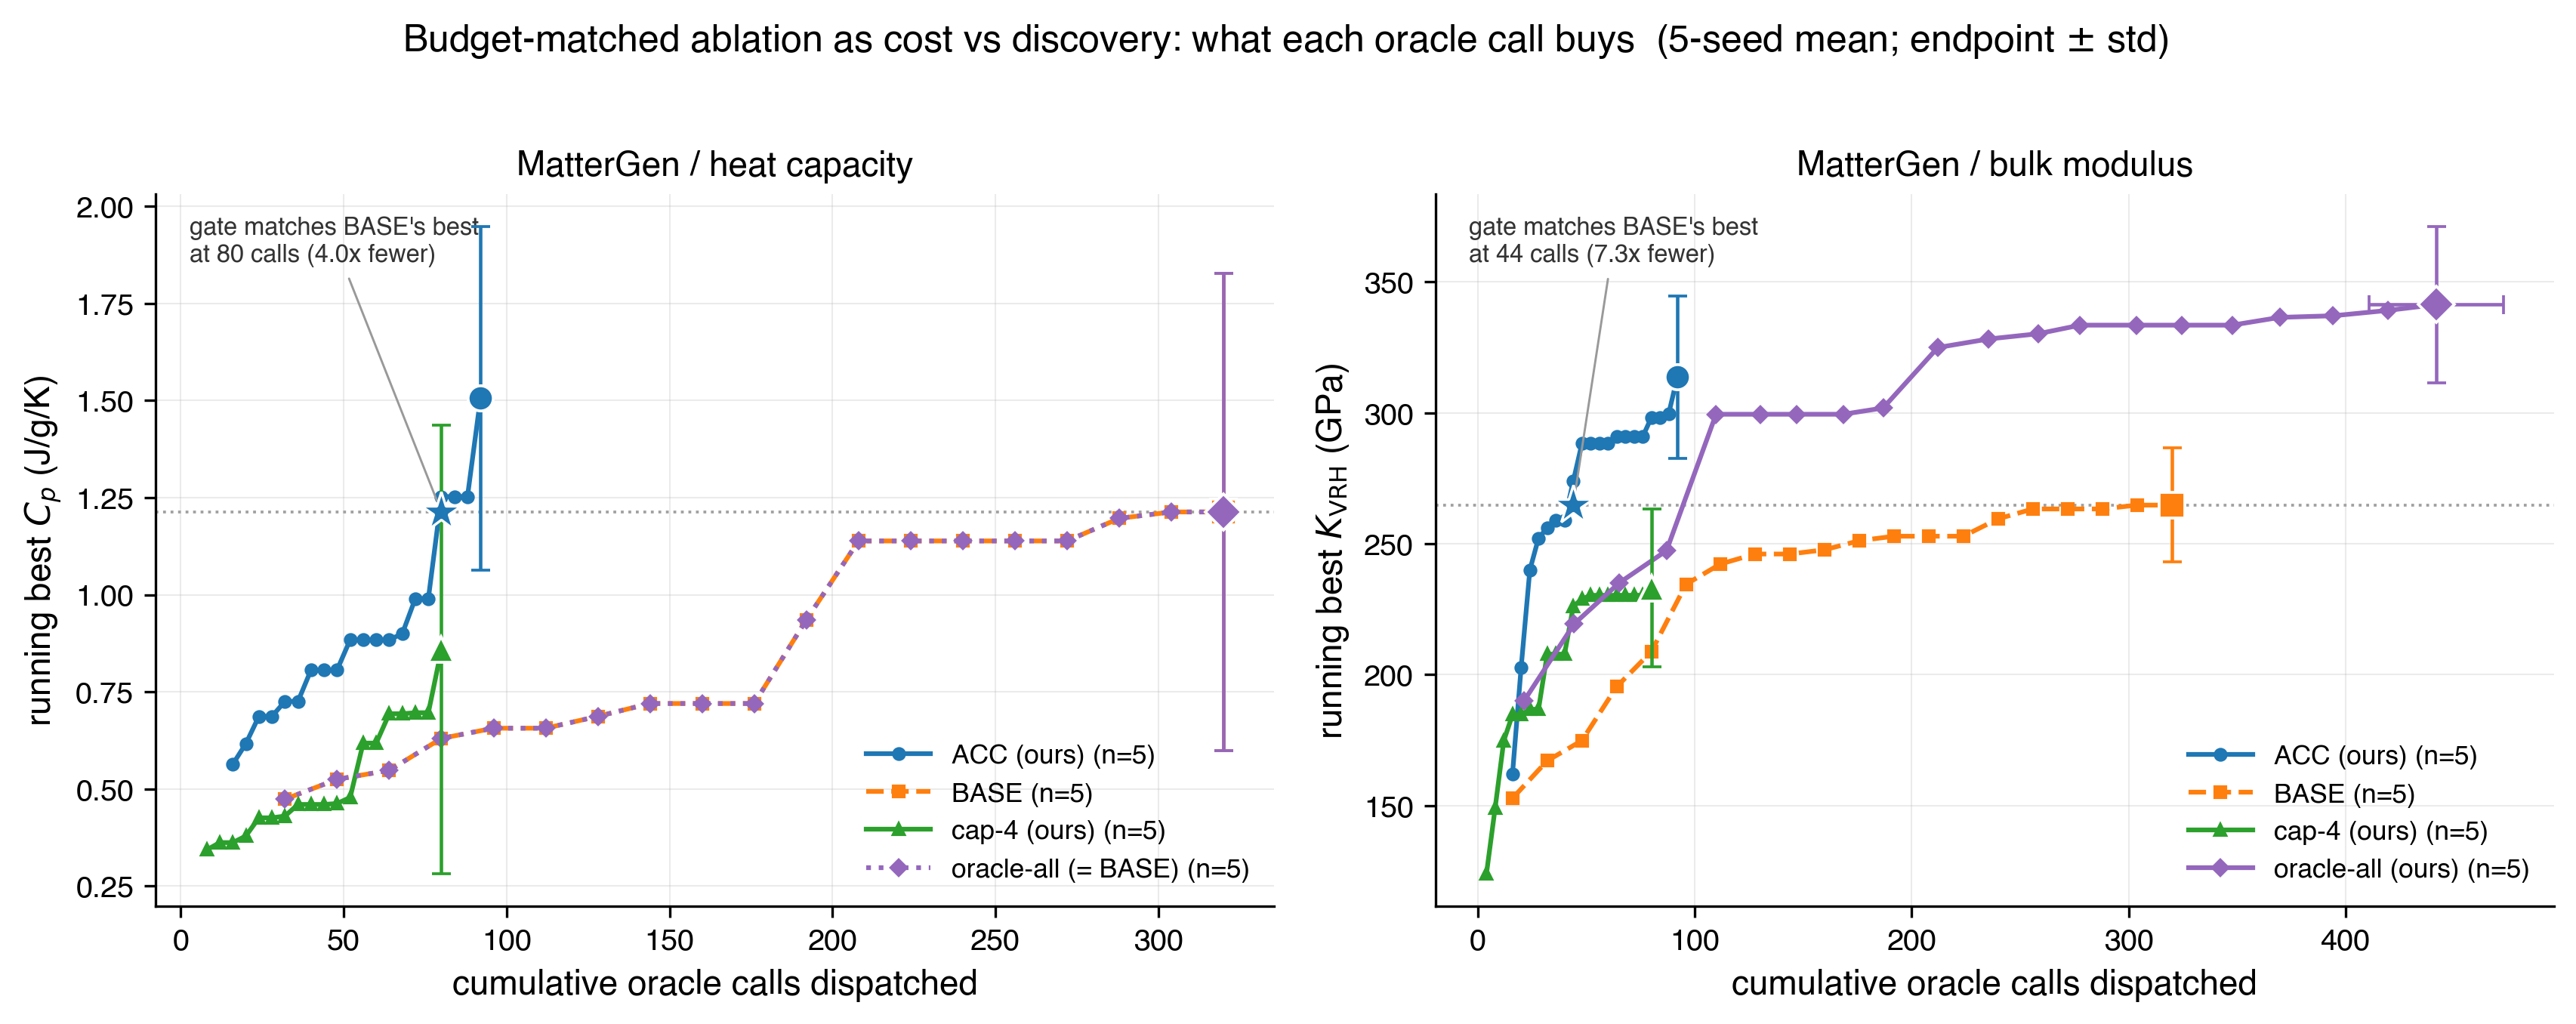
\includegraphics[width=0.98\linewidth]{figs/fig_mg_ablation_value_cost_dispatched.png}

\vspace{0.35cm}
\justifying
MatterGen with a fixed generation front end. Four arbitrary survivors
per cycle (cap-4) reach 233~GPa, against 314~GPa when the Gaussian
process chooses the four. Sending every survivor to the oracle reaches
341~GPa at 4.8 times the cost: the gate comes within 9\% of exhaustive
search at about one fifth of the calls.
\end{posterbox}

\end{postercol}

%======================= COLUMN 3 (right) =======================
\begin{postercol}{\colw\textwidth}

\begin{posterbox}{DFT Validation of Bulk Modulus}
\centering
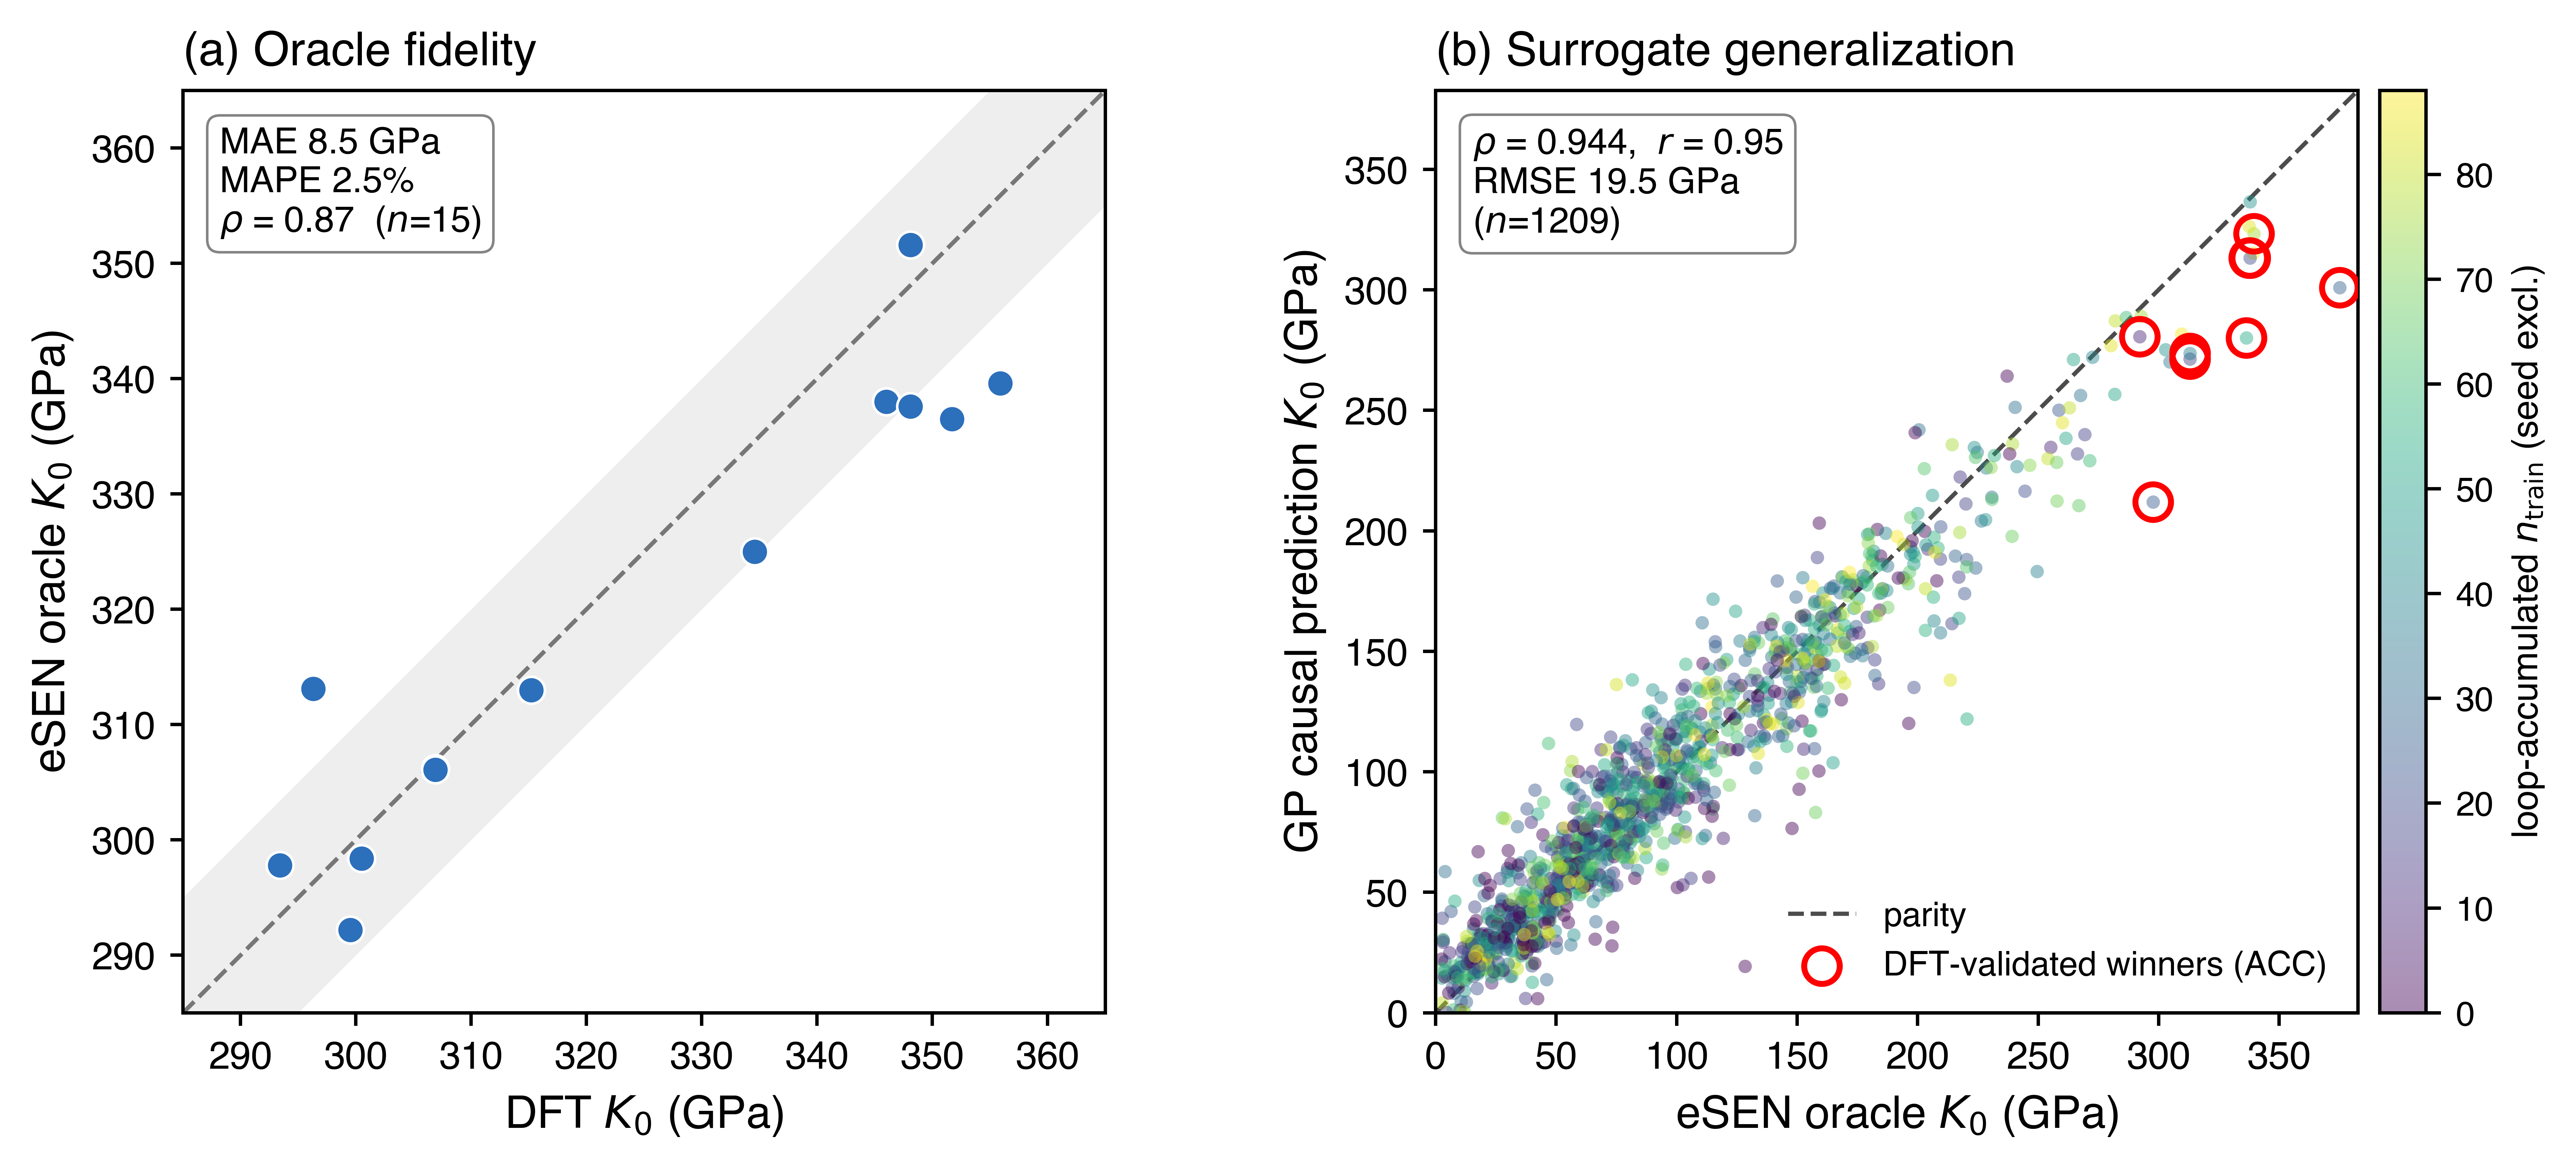
\includegraphics[width=\linewidth]{figs/fig_dft_bm_validation.png}

\vspace{0.35cm}
\justifying
(a) On 15 top structures recomputed with DFT, the learned oracle agrees
to 2.5\% (MAE 8.5~GPa). (b) Replayed causally, the Gaussian process ranks
1{,}209 unseen generated structures with Spearman $\rho = 0.94$, while
underpredicting the hardest extremes: it works as a ranker.
\end{posterbox}

\vfill

\begin{posterbox}{Novelty}
\justifying
None of the top structures match the warm-start pool under strict
structure matching (0 of 87 for heat capacity, 0 of 90 for bulk
modulus). The best bulk-modulus hit is an MoN polymorph in
$P\bar{6}m2$ at 375~GPa (354~GPa in DFT).
\end{posterbox}

\vfill

\begin{posterbox}{Conclusions}
\justifying
\begin{itemize}\setlength{\itemsep}{0.45cm}
\item A Gaussian-process gate matches or exceeds ungated fine-tuning
while holding oracle calls to a fixed budget.
\item The gain comes from ranking-based selection, not from spending
fewer calls.
\item ORB embeddings with a Gaussian process are the most reliable
surrogate across property classes.
\end{itemize}
\end{posterbox}

\end{postercol}
\end{columns}

\posterfooterrule
\gatefooter
  {Chen \textit{et al.}, MatInvent, arXiv:2511.03112 (2025).\quad
   Zeni \textit{et al.}, MatterGen, \textit{Nature} (2025).\\
   Luo \textit{et al.}, CrystalFlow, \textit{Nat.\ Commun.} (2025).\quad
   Joshi \textit{et al.}, ADiT, arXiv:2503.03965 (2025).\\
   Neumann \textit{et al.}, Orb, arXiv:2410.22570 (2024).\quad
   Fu \textit{et al.}, eSEN, arXiv:2502.12147 (2025).}
  {Supported by the Texas A\&M University System National Laboratories
   Office and Los Alamos National Laboratory (Joint Research Collaboration
   Program) and the U.S.\ DOE ARPA-E CHADWICK program (DE-AR0001988).
   Computing: Texas A\&M HPRC and NSF ACCESS allocation MAT250131 (ACES).}

\end{frame}
\end{document}
